\section*{In-order traversal}

One of the most important properties of a binary search tree is that
it maintains its elements in sorted order. The tree structure makes it
easy to find, add, and remove elements in their correct position, but
we haven't yet seen how to examine each element from smallest
to largest. This is called an \emph{in-order traversal}.

There are a few different ways to implement in-order traversal for a
binary search tree. In this lab, we'll be using a stack to keep track
of the nodes we still need to examine during traversal.  Specifically,
\textbf{whenever we follow the left child of a node, we push the node
  onto the stack} so we can come back to it later and visit its right
subtree. Here's an example showing each step of a traversal (visited
nodes have a green check mark next to them and the nodes on the stack
are circled):

\centerline{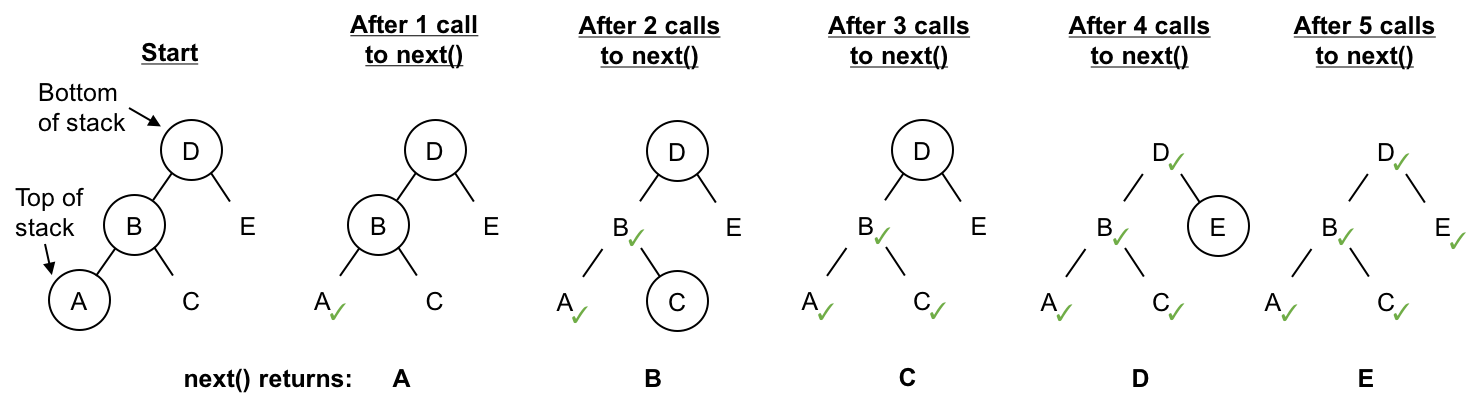
\includegraphics[scale=0.66]{\img/traversal.png}}

Notice how at each step, the next element we need to examine is at the
top of the stack. Also notice that the \lstinline'next()' function returns
each of the values in sorted order.

\begin{part}\TAGS{bst, stack, traverse-ds}
\begin{minipage}[t]{0.65\linewidth}
  Suppose a traversal is in the state shown to the right of this text
  (with only node C in the traversal stack). What will the stack
  contain after the traversal is advanced by one? By two? Which values
  will be returned?
\end{minipage}
\begin{minipage}[t]{0.3\linewidth}
  \rule{0em}{0ex}%
  \hfill
  \raisebox{-20ex}[0ex][20ex]{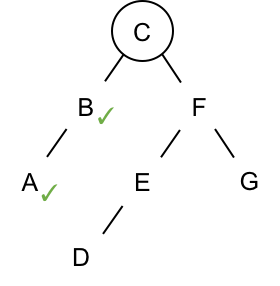
\includegraphics[scale=0.75]{\img/question.png}}
\end{minipage}

\end{part}
\vspace*{-2em}
\onePT[-8ex]
\begin{solution}
Advanced by 1:  (bottom) F, E, D (top)

Advanced by 2:  (bottom) F, E (top)
\end{solution}
